
% A LaTeX template for MSc Thesis submissions to 
% Politecnico di Milano (PoliMi) - School of Industrial and Information Engineering
%
% S. Bonetti, A. Gruttadauria, G. Mescolini, A. Zingaro
% e-mail: template-tesi-ingind@polimi.it
%
% Last Revision: October 2021
%
% Copyright 2021 Politecnico di Milano, Italy. NC-BY

\documentclass{Configuration_Files/PoliMi3i_thesis}

%------------------------------------------------------------------------------
%	REQUIRED PACKAGES AND  CONFIGURATIONS
%------------------------------------------------------------------------------

% CONFIGURATIONS
\usepackage{parskip} % For paragraph layout
\usepackage{setspace} % For using single or double spacing
\usepackage{emptypage} % To insert empty pages
\usepackage{multicol} % To write in multiple columns (executive summary)
\setlength\columnsep{15pt} % Column separation in executive summary
\setlength\parindent{0pt} % Indentation
\raggedbottom  

% PACKAGES FOR TITLES
\usepackage{titlesec}
% \titlespacing{\section}{left spacing}{before spacing}{after spacing}
\titlespacing{\section}{0pt}{3.3ex}{2ex}
\titlespacing{\subsection}{0pt}{3.3ex}{1.65ex}
\titlespacing{\subsubsection}{0pt}{3.3ex}{1ex}
\usepackage{color}

% PACKAGES FOR LANGUAGE AND FONT
\usepackage[english]{babel} % The document is in English  
\usepackage[utf8]{inputenc} % UTF8 encoding
\usepackage[T1]{fontenc} % Font encoding
\usepackage[11pt]{moresize} % Big fonts

% PACKAGES FOR IMAGES
\usepackage{graphicx}
\usepackage{transparent} % Enables transparent images
\usepackage{eso-pic} % For the background picture on the title page
\usepackage{subfig} % Numbered and caption subfigures using \subfloat.
\usepackage{tikz} % A package for high-quality hand-made figures.
\usetikzlibrary{}
\graphicspath{{./Images/}} % Directory of the images
\usepackage{caption} % Coloured captions
\usepackage{xcolor} % Coloured captions
\usepackage{amsthm,thmtools,xcolor} % Coloured "Theorem"
\usepackage{float}
\usepackage[outputdir=build,newfloat]{minted}
% STANDARD MATH PACKAGES
\usepackage{amsthm}
\usepackage{amssymb}
\usepackage{amsfonts}
\usepackage{bm}
\usepackage[overload]{empheq} % For braced-style systems of equations.
\usepackage{fix-cm} % To override original LaTeX restrictions on sizes

% PACKAGES FOR TABLES
\usepackage{tabularx}
\usepackage{longtable} % Tables that can span several pages
\usepackage{colortbl}

% PACKAGES FOR ALGORITHMS (PSEUDO-CODE)
\usepackage{algorithm}
\usepackage{algorithmic}

% PACKAGES FOR REFERENCES & BIBLIOGRAPHY
\usepackage[colorlinks=true,linkcolor=black,anchorcolor=black,citecolor=black,filecolor=black,menucolor=black,runcolor=black,urlcolor=black]{hyperref} % Adds clickable links at references
\usepackage{cleveref}
\usepackage[square, numbers, sort&compress]{natbib} % Square brackets, citing references with numbers, citations sorted by appearance in the text and compressed
\bibliographystyle{abbrvnat} % You may use a different style adapted to your field

% OTHER PACKAGES
\usepackage{listings}
\usepackage{pdfpages} % To include a pdf file
\usepackage{afterpage}
\usepackage{lipsum} % DUMMY PACKAGE
\usepackage{fancyhdr} % For the headers
\fancyhf{}

% Input of configuration file. Do not change config.tex file unless you really know what you are doing. 
% Define blue color typical of polimi
\definecolor{bluepoli}{cmyk}{0.4,0.1,0,0.4}

% Custom theorem environments
\declaretheoremstyle[
  headfont=\color{bluepoli}\normalfont\bfseries,
  bodyfont=\color{black}\normalfont\itshape,
]{colored}

% Set-up caption colors
\captionsetup[figure]{labelfont={color=bluepoli}} % Set colour of the captions
\captionsetup[table]{labelfont={color=bluepoli}} % Set colour of the captions
\captionsetup[algorithm]{labelfont={color=bluepoli}} % Set colour of the captions

\theoremstyle{colored}
\newtheorem{theorem}{Theorem}[chapter]
\newtheorem{proposition}{Proposition}[chapter]

% Enhances the features of the standard "table" and "tabular" environments.
\newcommand\T{\rule{0pt}{2.6ex}}
\newcommand\B{\rule[-1.2ex]{0pt}{0pt}}

% Pseudo-code algorithm descriptions.
\newcounter{algsubstate}
\renewcommand{\thealgsubstate}{\alph{algsubstate}}
\newenvironment{algsubstates}
  {\setcounter{algsubstate}{0}%
   \renewcommand{\STATE}{%
     \stepcounter{algsubstate}%
     \Statex {\small\thealgsubstate:}\space}}
  {}

% New font size
\newcommand\numfontsize{\@setfontsize\Huge{200}{60}}

% Title format: chapter
\titleformat{\chapter}[hang]{
\fontsize{50}{20}\selectfont\bfseries\filright}{\textcolor{bluepoli} \thechapter\hsp\hspace{2mm}\textcolor{bluepoli}{|   }\hsp}{0pt}{\huge\bfseries \textcolor{bluepoli}
}

% Title format: section
\titleformat{\section}
{\color{bluepoli}\normalfont\Large\bfseries}
{\color{bluepoli}\thesection.}{1em}{}

% Title format: subsection
\titleformat{\subsection}
{\color{bluepoli}\normalfont\large\bfseries}
{\color{bluepoli}\thesubsection.}{1em}{}

% Title format: subsubsection
\titleformat{\subsubsection}
{\color{bluepoli}\normalfont\large\bfseries}
{\color{bluepoli}\thesubsubsection.}{1em}{}

% Shortening for setting no horizontal-spacing
\newcommand{\hsp}{\hspace{0pt}}

\makeatletter
% Renewcommand: cleardoublepage including the background pic
\renewcommand*\cleardoublepage{%
  \clearpage\if@twoside\ifodd\c@page\else
  \null
  \AddToShipoutPicture*{\BackgroundPic}
  \thispagestyle{empty}%
  \newpage
  \if@twocolumn\hbox{}\newpage\fi\fi\fi}
\makeatother

%For correctly numbering algorithms
\numberwithin{algorithm}{chapter}

%----------------------------------------------------------------------------
%	NEW COMMANDS DEFINED
%----------------------------------------------------------------------------

% EXAMPLES OF NEW COMMANDS

%\renewcommand{\listingname}{Source code}
\newenvironment{code}{\captionsetup{type=listing}}{}
\SetupFloatingEnvironment{listing}{name=Source Code}

\newcommand{\bea}{\begin{eqnarray}} % Shortcut for equation arrays
\newcommand{\eea}{\end{eqnarray}}
\newcommand{\e}[1]{\times 10^{#1}}  % Powers of 10 notation

%----------------------------------------------------------------------------
%	ADD YOUR PACKAGES (be careful of package interaction)
%----------------------------------------------------------------------------

%----------------------------------------------------------------------------
%	ADD YOUR DEFINITIONS AND COMMANDS (be careful of existing commands)
%----------------------------------------------------------------------------

%----------------------------------------------------------------------------
%	BEGIN OF YOUR DOCUMENT
%----------------------------------------------------------------------------

\begin{document}

\fancypagestyle{plain}{%
\fancyhf{} % Clear all header and footer fields
\fancyhead[RO,RE]{\thepage} %RO=right odd, RE=right even
\renewcommand{\headrulewidth}{0pt}
\renewcommand{\footrulewidth}{0pt}}

%----------------------------------------------------------------------------
%	TITLE PAGE
%----------------------------------------------------------------------------

\pagestyle{empty} % No page numbers
\frontmatter % Use roman page numbering style (i, ii, iii, iv...) for the preamble pages

\puttitle{
	title=Mobile applications State Management in Flutter, % Title of the thesis
	name=Lorenzo Ventura, % Author Name and Surname
	course= Computer Science - Ingegneria Informatica, % Study Programme (in Italian)
	ID  = 906003,  % Student ID number (numero di matricola)
	advisor= Prof. Luciano Baresi,
	coadvisor=,% Supervisor name
	academicyear={2021-2022}  % Academic Year
} % These info will be put into your Title page 

%----------------------------------------------------------------------------
%	PREAMBLE PAGES: ABSTRACT (inglese e italiano), EXECUTIVE SUMMARY
%----------------------------------------------------------------------------
\startpreamble
\setcounter{page}{1} % Set page counter to 1

% ABSTRACT IN ENGLISH
\chapter*{Abstract} 
Abstract
\\
\\
\textbf{Keywords:} here, the keywords, of your thesis % Keywords

% ABSTRACT IN ITALIAN
\chapter*{Abstract in lingua italiana}
Qui va l'Abstract in lingua italiana della tesi seguito dalla lista di parole chiave.
\\
\\
\textbf{Parole chiave:} qui, vanno, le parole chiave, della tesi % Keywords (italian)

%----------------------------------------------------------------------------
%	LIST OF CONTENTS/FIGURES/TABLES/SYMBOLS
%----------------------------------------------------------------------------

% TABLE OF CONTENTS
\thispagestyle{empty}
\tableofcontents % Table of contents 
\thispagestyle{empty}
\cleardoublepage

%-------------------------------------------------------------------------
%	THESIS MAIN TEXT
%-------------------------------------------------------------------------
% In the main text of your thesis you can write the chapters in two different ways:
%
%(1) As presented in this template you can write:
%    \chapter{Title of the chapter}
%    *body of the chapter*
%
%(2) You can write your chapter in a separated .tex file and then include it in the main file with the following command:
%    \chapter{Title of the chapter}
%    \input{chapter_file.tex}
%
% Especially for long thesis, we recommend you the second option.

\addtocontents{toc}{\vspace{2em}} % Add a gap in the Contents, for aesthetics
\mainmatter % Begin numeric (1,2,3...) page numbering

% --------------------------------------------------------------------------
% NUMBERED CHAPTERS % Regular chapters following
% --------------------------------------------------------------------------
\chapter*{Introduction}


Introduction   

\section{General Background}
input{./Sections/GeneralBackground.tex}

\section{The experiment  the model}
\label{sec:general_overview}
input{./Sections/GeneralOverview.tex}

\label{ch:introduction}%

\chapter{State management solutions}
\label{ch:chapter_one}%
here i will present some main concepts and functionalities of the state management solutions proposed. This chapter will be filled with the information contained in the other word file i sent you.
\section{SetState and InheritedWidget/InheritedModel}
\label{sec:setState}

...
\section{Redux}
\label{sec:Redux}

...
\section{BLoc}
\label{sec:BLoC}

...a
\section{MobX}
\label{sec:MobX}

...
\section{GetX}
\label{sec:GetX}

...

\chapter{The Todo app}
\label{ch:chapter_two}
This chapter is devoted to the implementation of a mobile application regarding the management of a number of todos. It is developed using the state managemenent solutions proposed in Chapter 1. For every solution, three different development processes are carried out. Moreover, a series of measurements ,concerning the volume of the code and the effort spent, will be collected.
\section{General overview}
\label{sec:general_overview}
This section explains in details the three development processes and the resulting application. These processes consist in the implementation of the main functionalities, in the addition of new ones and in some performance optimizations.
\subsection{Base functionalities}
\label{subsec:base_functionalities}

This part of the development process aims to realize a skeleton of the application and its main functionalities. The output of the process will be and application offering the possibility to visualize and partially handle a list of todos. It is composed by a single page: the HomePage. The HomePage is made of an AppBar and two tabs: the \textit{todos} tab and the \textit{stats} tab. \\
The \textit{todos} tab visualizes the list of todos. It is possible to filter todos using a DropdownButton widget situated in the top right corner, inside the AppBar. 
The available filter values are:
\begin{itemize}
    \item All (visualizes completed and pending todos)
    \item Completed (visualizes completed todo only)
    \item Not Completed (visualizes pending todos only)
\end{itemize}
The list of todos is visualized using a TodoView component widget. The elements contained in the TodoView component are called TodoItems. TodoItem widgets visualize the name, the description and the completion of a specific todo using two Text widgets and a Checkbox widget. It is possible to use the checkbox in order to mark a todo as completed or to mark it as pending depending on its current state. \\
The \textit{stats} tab visualizes the number of completed todos through a Text widget.
In the lower part, a TabSelector widget allow to switch from tabs.

\begin{figure}[H]
    \centering
    \subfloat[\textit{todos} tab runtime UI\label{fig:todos_tab_tree}]{
        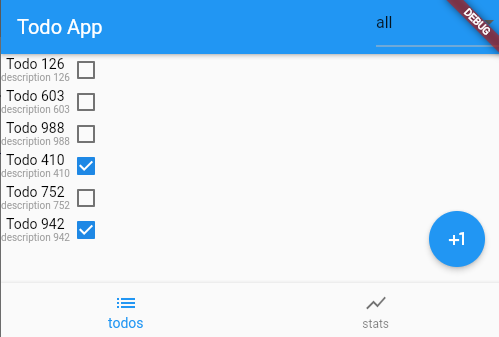
\includegraphics[scale=0.5]{Images/shot_runtime_todoapp_todos.png}
    }
    \quad
      \subfloat[\textit{stats} tab runtime UI.\label{fig:todos_tab_UI}]{
        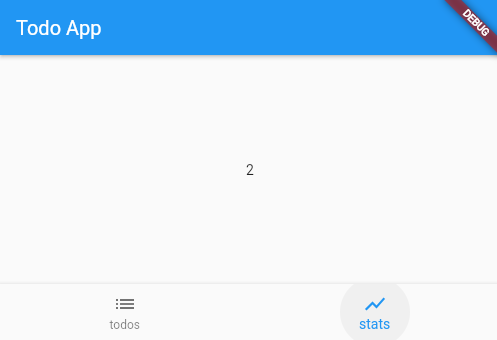
\includegraphics[scale=0.5]{Images/shot_runtime_todoapp_stats.png}
    }
    \caption{Shows the HomePage's UI }
    \label{fig:todos_tab}
\end{figure}

\subsection{Adding new features}
\label{subsec:adding_new_features}


Once basic functionalities got implemented a few more will be added. This part of the development process is divided into two subpart. Both of them aims to add a single new feature.

\paragraph{The Add todo Feature} \mbox{} \\
\label{par:add_todo_feature_explanation}
 The first subpart of the features addition process aims to add the possibility to create new Todos. This feature will utilize the FloatingActionButton already present in the skeleton of the app in the bottom right corner to push the AddTodoPage. In the AddTodoPage will be possible to compile some TextField widget and use a TextButton to actually create the new todo.
 
 
\paragraph{The Update feature} \mbox{} \\
\label{par:update_todo_feature_explanation}
The second subpart of the features addition process aims to add the possibility to tap on a specific TodoItem to navigate to the UpdateTodoPage where two TextFields and a TextButton button will show. Once inserted a new name and/or a new description for the todo, clicking on the confirm button the UpdateTodoPage route will be popped and the todo will be updated. 

\subsection{Renders optimization}
\label{subsec:renders_optimization}

This part of the development process aims to perform some optimizations in terms of UI rendering and memory consumption. In particular, the code will be refactored in order to use the least UI renders possible and ,in other words, to call the least \textit{build} methods possible. The focus is on the TodoView and TodoItem widgets. The TodoView widget should be rendered again only after a structural change in the \textit{filteredTodos} list. A structural change is intended as a mutation of the length of the list or a substitution of its internal elements. Basically, a structural change occurs when a new todo is added or removed from the list or when the filter changes. If the change concerns a single todo (e.g. when its internal state is changed using the checkbox or the update feature)it is considered a non-structural change. The main difference is that, a structural change, needs to rebuild the entire TodoView ,instead, a non-structural change can rebuild only a subpart (the particular TodoItem). This because , when a structural change occurs, more than one TodoItem is affected and ,the most convinient way to mutate them all consistently ,is to rebuild the entire TodoView widget. Moreover, addind , deleting and substituting a TodoItem (and consequently add/delete/substitute a child to the TodoView tree node) is only possible by the parent widget and not by widgets on the same tree level. A non-structural change ,instead, affects only a specific TodoItem/child and so, it is possibile to rebuild the single element only. Those optimizations are not really necessary in this scenario. The implemented application is ,indeed, very simple and do not need this kind of improvements at all. This is just an experiment in order to define which solution performs better at handling optimizations and to give an adjunctive prospective in the final comparison.


\section{Implementation}
\label{sec:implementation}
in this section the development process with different State Management solutions will be presented.

\subsection{Shared project structure and files}
\label{subsec:SharedStructureTodo}
In order to make comparisons even more fair , the code about the application's core and UI is shared between different solution's implementations. This subsection presents the shared code in details. Some parts of the shared code can change from one implementation to another in order to adapt to the solution. However, changes to this structure are kept minimal. And the same is for the UI. It uses the least widget and visual features possible. In the Figure \ref{fig:todo_app_shared_folder_structure} the shared folder's and file's structure is shown. Subsequent paragraphs exaplains how models, pages, components and the repository are implemented. 

		
		\begin{figure}[H]
		    \centering
		    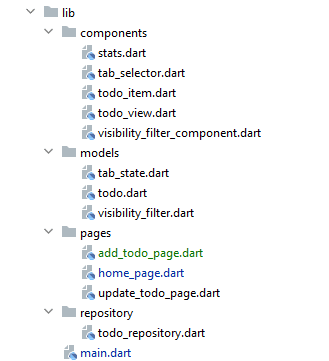
\includegraphics[width=0.6\textwidth]{Images/folder_structure.png}
		    \caption{Todos app skeleton's folders structure.}
		    \label{fig:todo_app_shared_folder_structure}
		\end{figure}
		
		
		
\paragraph{The application's Root} \mbox{} \\
		\label{par:todo_app_application_root}
The root widget of the application is called MyApp.
It is a stateful widget composed by a MaterialApp. Inside the MaterialApp, three routes are defined : the HomePage , the UpdateTodoPage and the AddTodoPage. The \textit{inizialRoute} is set to the HomePage as deafult. Inside the \textit{main} function the MyApp widget is passed to the \textit{runApp} method at the application's start.
		
		\begin{code}
		
		\mbox{}\\
		\captionof{listing}{Todo app - MaterialApp and main function definition} \mbox{}
		
		\label{code:2.1}

	\begin{minted}{dart}
	
void main() {
  runApp(const MyApp());
}

class MyApp extends StatefulWidget {
  const MyApp({Key? key}) : super(key: key);

  @override
  State<MyApp> createState() => _MyAppState();
}

class _MyAppState extends State<MyApp> {

  @override
  Widget build(BuildContext context) {
    return MaterialApp(
      initialRoute: "/",
      routes: {
        "/": (context) => const HomePage(),
        "/updateTodo": (context) => UpdateTodoPage(),
        "/addTodo": (context) => AddTodoPage(),

      },
    );
  }
}	
	\end{minted}
	
\end{code}	
	
	\paragraph{Models and Repository} \mbox{} \\
	\label{par:todo_app_models_and_repository}
as show in code \ref{code:c-code} HomePage's tabs are only two : \textit{todos} and \textit{stats}. In the \textit{todos} tab todos are visualized. In the \textit{stats} tab ,instead, some numerical recap of the todos is visualized. They are defined using an enumeration for simplicity.

	\mbox{}\\
	\begin{code}
	
	\captionof{listing}{Todo app - TabState model definition}
			\label{code:2.2}

	 \mbox{}
	\begin{minted}{dart}
	
	enum TabState{
	 todos,stats
	}
	
	
	\end{minted}
	\end{code}
	\mbox{}
	
Filters for the \textit{filteredTodos} list are modelled by an enumeration too. They can take three values: \textit{all, notCompleted, completed}.
	
	\mbox{}\\
\begin{code}	
	\captionof{listing}{Todo app - VisibilityFilter model definition} \mbox{}\\
			\label{code:2.3}

	\begin{minted}{dart}
	
	enum VisibilityFilter{
	 completed,notCompleted,all
	}
	
	
	\end{minted}
	\end{code}
	\mbox{}
	
It's not possible to give a common implementation of the Todo model matching every solution. Todo model ,indeed, change in different implementations. The sharable structure of the model ,however, can defined as below RIFERIMENTO. (
	\mbox{}\\
	\begin{code}
	
	\captionof{listing}{Todo app - Todo model definition} \mbox{}
\label{code:2.4}
	\begin{minted}{dart}
	
	@immutable
	class Todo {
	  final int id;
	  final String name;
	  final String description;
	  final bool completed;
	
	  const Todo(
	      {required this.id,
	      required this.name,
	      required this.description,
	      required this.completed});
	
	  @override
	  bool operator ==(Object other) {
	    return (other is Todo) &&
	        other.description == description &&
	        other.name == name &&
	        other.id == id &&
	        other.completed == completed;
	  }
	
	  @override
	  String toString() {
	    return "{ id: $id  completed: $completed}";
	  }
	
	  @override
	  // TODO: implement hashCode
	  int get hashCode => super.hashCode;
	}
	
	\end{minted}
	\end{code}
	\mbox{}
	
	
The TodoRepository class simulate todos's fetching from a Database. It has two static methods. These methods are asynchronous and have a duration of 2 seconds to give the impression of a real asynchronous operation. The method \textit{loadTodos} , in particular , populate a list with six new todos after the generation of their unique ID's. Subsequently, after 2 seconds, returns it to the caller.
	
	\mbox{}\\
	\begin{code}
	\captionof{listing}{Todo app - TodoRepository definition} \mbox{}
			\label{code:2.5}

	\begin{minted}{dart}
	
	class TodoRepository {
	  static Future<List<Todo>> loadTodos() async {
	    Random rand = Random();
	    List<Todo> todos = [];
	    List<int> ids = [];
	    while (ids.length < 6) {
	      int newInt = rand.nextInt(1000)+2;
	      if (!ids.contains(newInt)) {
	        ids.add(newInt);
	      }
	    }
	    todos = ids
	        .map((number) => Todo(
	            id: number,
	            name: "Todo " + number.toString(),
	            description: "description " + number.toString(),
	            completed: rand.nextBool()))
	        .toList();
	
	    await Future.delayed(const Duration(seconds: 2));
	    return todos;
	  }
	
	  static Future<void> saveTodos(List<Todo> todos) async {
	    await Future.delayed(const Duration(seconds: 2));
	  }
	}
	
	
	\end{minted}
	\end{code}
	\mbox{}
	
	
	\paragraph{Pages} \mbox{} \\
	\label{par:todo_app_pages}
Homepage uses a simple Scaffold widget. The AppBar contains a VisibilityFilterComponent only when the tab is set to \textit{todos}. The body can change from \textit{todos} tab to \textit{stats} tab using the BottomNaviagationBar (the TabSelector). An empty FloatingActionButton is also present for future implementation.
	(note: some small pieces could change in different solution’s implementation. in the above example the tab changing is implemented through setState but it will not be always the case. Also ,the HomePage, can be muted to Stateless widget in other implementations.).
	
	\mbox{}\\
	\begin{code}
	\captionof{listing}{Todo app - HomePage definition} \mbox{}
			\label{code:2.6}

	\begin{minted}{dart}
	class HomePage extends StatefulWidget {
	  const HomePage({Key? key}) : super(key: key);
	
	  @override
	  State<HomePage> createState() => _HomePageState();
	}
	
	class _HomePageState extends State<HomePage> {
	  TabState tab = TabState.todos; 
	
	  @override
	  Widget build(BuildContext context) {
	    return Scaffold(
	          appBar: AppBar(
	            actions: [
	              tab == TabState.todos
	                  ? const VisibilityFilterComponent()
	                  : Container()
	            ],
	            title: const Text("Todo App"),
	          ),
	          body: tab == TabState.todos ? const TodoView() : const Stats(),
	          bottomNavigationBar: TabSelector(
	            currTab: tab,
	            onTabChange:,
	          ),
	          floatingActionButton: tab == TabState.todos
	              ? FloatingActionButton(
	                  child: const Icon(Icons.plus_one),
	            onPressed: () {},
	          ) : null,
	        )
	    );
	  }
	}
	
	
	\end{minted}
	\end{code}
	\mbox{}
	
	
	The UpdateTodoPage uses a Scaffold widget. The body is filled with a Column with two TextFields and a TextButton inside. The TextButton is left empty for future implementation.
	
	\mbox{}\\
	\begin{code}
	\captionof{listing}{Todo app - UpdatePage definition} \mbox{}
			\label{code:2.7}
	\begin{minted}{dart}
	class UpdateTodoPage extends StatefulWidget {
	  final Todo todo;
	  final void Function(String,String) callback;
	
	  const UpdateTodoPage({Key? key, required this.todo,required this.callback}) : super(key: key);
	
	  @override
	  State<UpdateTodoPage> createState() => _UpdateTodoPageState();
	}
	
	class _UpdateTodoPageState extends State<UpdateTodoPage> {
	  final textControllerName = TextEditingController();
	  final textControllerDesc = TextEditingController();
	
	  @override
	  Widget build(BuildContext context) {
	
	    return Scaffold(
	        appBar: AppBar(
	          title: Text("Update Todo"+widget.todo.name),
	        ),
	        body: Column(
	          children: [
	            TextField(
	              controller: textControllerName,
	              decoration: const InputDecoration(
	                  border: OutlineInputBorder(), hintText: 'Enter a new name'),
	            ),
	            TextField(
	              controller: textControllerDesc,
	              decoration: const InputDecoration(
	                  border: OutlineInputBorder(), hintText: 'Enter a new description'),
	            ),
	            TextButton(onPressed: () {},
	            child: const Text("Confirm"))
	          ],
	        ));
	  }
	
	  @override
	  void dispose() {
	    textControllerName.dispose();
	    textControllerDesc.dispose();
	    super.dispose();
	  }
	}
	
	\end{minted}
	\end{code}
	\mbox{}
	
	
	
	The AddTodoPage uses a Scaffold widget. The body is filled with Column with two TextField widgets and a TextButton widget inside. The TextButton is left empty for future implementation.
	
	\mbox{}\\
	\begin{code}
	\captionof{listing}{Todo app - AddTodoPage definition} \mbox{}
			\label{code:2.8}

	\begin{minted}{dart}
	
	class AddTodoPage extends StatefulWidget {
	
	  final void Function(String,String) addTodoCallback;
	
	  const AddTodoPage({Key? key, required this.addTodoCallback}) : super(key: key);
	
	  @override
	  State<AddTodoPage> createState() => _AddTodoPageState();
	}
	
	class _AddTodoPageState extends State<AddTodoPage> {
	  final textControllerName = TextEditingController();
	  final textControllerDesc = TextEditingController();
	
	  @override
	  Widget build(BuildContext context) {
	
	    return Scaffold(
	        appBar: AppBar(
	          title: const Text("Add Todo"),
	        ),
	        body: Column(
	          children: [
	            TextField(
	              controller: textControllerName,
	              decoration: const InputDecoration(
	                  border: OutlineInputBorder(), hintText: 'Enter a name'),
	            ),
	            TextField(
	              controller: textControllerDesc,
	              decoration: const InputDecoration(
	                  border: OutlineInputBorder(), hintText: 'Enter a description'),
	            ),
	            TextButton(onPressed: () {}
	            , child: const Text("Create"))
	          ],
	        ));
	  }
	
	  @override
	  void dispose() {
	    textControllerName.dispose();
	    textControllerDesc.dispose();
	    super.dispose();
	  }
	}
	
	\end{minted}
	\end{code}
	\mbox{}
	
	
	\paragraph{Components} \mbox{} \\
	\label{par:todo_app_components}
	Components are widgets created with a specific aims.
	TodoView component take care to visualize a list of todos. Todos are accessed in different ways depending on the implementation. TodoView uses a ListView widget. \textit{itemCount} and \textit{itemBuilder} fields are left empty for future implementation.
	
	\mbox{}\\
	\begin{code}
	\captionof{listing}{Todo app - TodoView definition} \mbox{}
			\label{code:2.9}
	\begin{minted}{dart}
	class TodoView extends StatelessWidget {
	
	  const TodoView({Key? key}) : super(key: key);
	
	  @override
	  Widget build(BuildContext context) {
	    print("Building TodoView");
	
	
	    return ListView.builder(
	      itemCount:,
	      itemBuilder: (context, index) {
	        return TodoItem(
	          
	        );
	      },
	    );
	  }
	}
	
	\end{minted}
	\end{code}
	\mbox{}
	
	
	TodoItem is a component that take care to visualize a specific todo. TodoItem is a stateless widget. It uses two Text widgets to display the todo's information and a Checkbox to change the todo’s completion. It is wrapped in a InkWell widget to make is responsive to taps. Functions are left empty for future implementation.
	
	\mbox{}\\
	\begin{code}
	\captionof{listing}{Todo app - TodoItem definition} \mbox{}
			\label{code:2.10}
	\begin{minted}{dart}
	class TodoItem extends StatelessWidget {
	  final Todo todo;
	
	  const TodoItem({Key? key, required this.id}) : super(key: key);
	
	  @override
	  Widget build(BuildContext context) {
	    print("Building Todo Item \$todo");
	
	    return InkWell(
	      onTap: () {
	        Navigator.pushNamed(context, "/updateTodo");
	      },
	      child: Row(
	        children: [
	          Column(
	            children: [
	              Text(todo.name,
	                  style: const TextStyle(fontSize: 14, color: Colors.black)),
	              Text(todo.description,
	                  style: const TextStyle(fontSize: 10, color: Colors.grey)),
	            ],
	          ),
	          Checkbox(
	              value: todo.completed,
	              onChanged: (value) {}),
	        ],
	      ),
	    );
	  }
	}
	
	\end{minted}
	\end{code}
	\mbox{}
	
	
	TabSelector component provides a way to switch from tabs. Tabselector uses a BottomNavigationBar with as many BottomNavigationBarItems as TabState.values (in our case two). Functions's fields are left empty for future implementation.
	
	\mbox{}\\
	\begin{code}
	\captionof{listing}{Todo app - TabSelector definition} \mbox{}
			\label{code:2.11}
	\begin{minted}{dart}
	class TabSelector extends StatelessWidget {
	
	
	  const TabSelector(
	      {Key? Key})
	      : super(key: key);
	
	  @override
	  Widget build(BuildContext context) {
	    print("Building Tab Selector");
	
	    return BottomNavigationBar(
	      currentIndex: ,
	      onTap: (){},
	      items: TabState.values
	          .map((tab) => BottomNavigationBarItem(
	                label: describeEnum(tab),
	                icon: Icon(
	                  tab == TabState.todos ? Icons.list : Icons.show_chart,
	                ),
	              ))
	          .toList(),
	    );
	  }
	}
	
	\end{minted}
	\end{code}
	\mbox{}
	
	VisibilityFilterComponent uses a DropdownButton with as many DropdownMenuItems as VisibilityFilter.values (in our case three). Function fields are left empty for future implementation.
	
	\mbox{}\\
	\begin{code}
	\captionof{listing}{Todo app - VisibilityFilterSelector definition} \mbox{}
			\label{code:2.12}
	\begin{minted}{dart}
	class VisibilityFilterComponent extends StatelessWidget {
	
	  const VisibilityFilterComponent(
	      {Key? key})
	      : super(key: key);
	
	  @override
	  Widget build(BuildContext context) {
	    print("Building Visibility filter");
	    return DropdownButton<VisibilityFilter>(
	      value:,
	      items: VisibilityFilter.values.map((filter) {
	        return DropdownMenuItem<VisibilityFilter>(
	            child: Text(describeEnum(filter)), value: filter);
	      }).toList(),
	      onChanged: (filter) {
	       
	      },
	    );
	  }
	}
	\end{minted}
	\end{code}
	\mbox{}
	
	Stats component takes care to visualize some numerical representation of the list of todos. Stats component is a Stateless widget composed by Text widget showing stats value.
	
	\mbox{}\\
	\begin{code}
	\captionof{listing}{Todo app - Stats definition} \mbox{}
		\label{code:2.13}
	\begin{minted}{dart}
		

	class Stats extends StatelessWidget {
  const Stats({Key? key}) : super(key: key);

  @override
  Widget build(BuildContext context) {
    print("Building Stats");

    return Center(
        child: Text());
  }
}
	\end{minted}
	\end{code}
	\mbox{}
	
	


\subsection{Inherited widget/model and SetState implementation}
This section implements the Todo application using two standard tools the Flutter framework provides in order to handle the state. These tools are InheritedWidgets and InheritedModels plus the usual \textit{setState} function.

\subsubsection{Base functionalities} 
\label{par:todo_app_inherited_widget_base_app}

\paragraph{The core state - }
\label{subpar:todo_app_inherited_widget_core_state}
In order to use InheritedWidget's functionalities, a new class must be defined and extended with InheritedWidget class. For our purpose, a single class will be enough to contain all the application's state. This new class is called \textit{TodoInheritedData}.
\begin{code}
\mbox{}
\captionof{listing}{Todo app - InheritedWidget - extension to InheritedWidget} \mbox{}
		\label{code:2.14}
\begin{minted}[bgcolor=bluepoli!10]{dart}
class TodoInheritedData extends InheritedWidget{
\end{minted}
\mbox{}
\end{code}

The application's state is composed by: a list of Todos, a VisibilityFilter , an Int for the stats ( for conciseness it will represent the number of completed todos) and a filtered list of todos which contains the todos matching the visibility filter. Inside the constructor, final variables are initialized with their corresponding arguments, moreover, \textit{stats} and \textit{filteredTodos} list are computed. 
\mbox{}\\
\begin{code}
\captionof{listing}{Todo app - InheritedWidget- TodoInheritedData implementation} 
\mbox{}
\label{code:2.15}
\begin{minted}[bgcolor=bluepoli!10]{dart}

class TodoInheritedData extends InheritedWidget{
 final List<Todo> todos;
 final List<Todo> filteredTodos;
 final VisibilityFilter filter;
 final int stats;
 
TodoInheritedData(
    { 
    Key? key,
    required this.todos,
    required this.filter,
    required Widget child})
    : stats = todos.length, //computing stats
      filteredTodos = filterTodo(todos, filter),//computing filtered list
      super(child: child, key: key);
}
\end{minted}
\end{code}
\mbox{}\\
\textit{filterTodos} function is just a function taking a list of todos and a visibility filter and returning the filtered list. Important to notice is the fact that a \textit{child} widget must also be provided in the constructor. This because TodoInheritedData is nothing else than a widget itself that wraps the state and makes it accessible down the tree.

TodoInheritedData widget is stateless. It cannot be changed (every value is final) and a new TodoInheritedData widget must be provided when a data change occurs. 
The \textit{updateShouldNotify }method must be overridden inside the TodoInheritedData class. This method belongs to the InheritedWidget class and its override is mandatory. It helps avoiding useless UI rebuilding when a new state, without actual data changes, occurs. Once a TodoInheritedData widget is replaced with a new one, the new widget takes care of calling the \textit{updateShouldNotify }method and deciding whether is necessary to notify changes in the subtree. If the method returns \textit{true }, the subtree is rebuilt, if  it returns \textit{false}, instead, it is not.
\mbox{}\\
\begin{code}
\captionof{listing}{Todo app - InheritedWidget - TodoInheritedData's \textit{ updateShouldNotify} method override} \mbox{}

\label{code:2.17}
\begin{minted}[bgcolor=bluepoli!10]{dart}

@override
bool updateShouldNotify(TodoInheritedData oldWidget) {
  return !listEquals(oldWidget.filteredTodos, filteredTodos);
}
\end{minted}
\end{code}

\textit{listEquals }function is provided by the Dart language. It takes two lists and compares them element by element, returning true if all elements are equal. In the Source Code \ref{code:2.17}, it takes as parameters the old \textit{filteredTodos} list (the one belonging to the old widget)  and the new \textit{filteredTodos} list and compares them. In case no changes were performed it returns \textit{true} and leads the \textit{updateShouldNotify }function to return \textit{false}, leaving the subtree unchanged.\\
InheritedWidget class requires also the \textit{of} method override. The \textit{of }method makes the instance of the TodoInheritedData class accessible down the tree. It is a static method (it can be called without istantiating any TodoInheritedData object) and returns the instance of the nearest TodoInheritedData widget up in the tree. It extracts the instance from the current \textit{context} object using the method called \textit{dependOnInheritedWidgetOfExactType} provided by the Flutter framework. In case no TodoInheritedData widget is found it raises a runtime error.
\mbox{}
\begin{code}
\captionof{listing}{Todo app - InheritedWidget - TodoInheritedData \textit{of} method override} \mbox{}
\label{code:2.18}
\begin{minted}[bgcolor=bluepoli!10]{dart}

static TodoInheritedData? of(BuildContext context) {
 final TodoInheritedData? result =
  context.dependOnInheritedWidgetOfExactType<TodoInheritedData>(); 
assert(result != null, 'No TodoInheritedData found in context');
return result;
}
\end{minted}
\end{code}

TodoInheritedData widget is now ready to be used. In the overall it is a container for our state. It makes the state accessible in the subtree but, is not clear yet who is really filling it with the correct informations. TodoInheritedData widget represents the state of the appplication in a given moment. It cannot change its internal values neither substitute itself with another instance. In practice , what happends, is that a stateful widget is created. This stateful widget contains the state and bothers to create a new instance of the TodoInheritedData widget every time the state changes. Everytime its internal state is changed (using \textit{setState}), indeed, a new instance of TodoInheritedData widget is produced and substituted with the old one. In this way, changes are reported to the subtree which sees a different image of the state and rebuild with it. I personally did not appreciate this adjunctive data cache layer InheritedWidget introduces. On one way it is simple and works really well for its purpose , on the other hand it introduces a new level of data caching. The concept of data caching will be explained a bit more in details later but ,for the moment ,we can say that the application's state is not exactly atomic/unique. What is seen by the subtree is a screenshot of the state and not the state itself. The real state is contained in the stateful widget. It is important, though, that the real state and the screenshot provided in the subtree are well syncronized. A bad syncronization can produce inconsistency in what is visualized and the information contained in the internal state. More in general, it can be said , that the more data caching levels are introduced the harder it gets to efficiently syncronize them. It is clear that ,in our scenario ,this problem does not really show up. Or better, it will in the optimization part but ,in that case, InheritedWidget tool is used with a purpose that goes behoind its real usage. Anyway, it is possible that different widgets sees different screenshots of the data and the bigger the application grows the higher will be the probability that this scenario show up. Now that the background is a bit clearer the implementation process can continue. As mentioned above, a new stateful widget must be created. This new stateful widget is called \textit{TodoProvider.} It has two variables representing the state: a list of todos and a filter. (the rest of the state is computed at each TodoInheritedData creation)
\mbox{}\\
\begin{code}
\captionof{listing}{Todo app - InheritedWidget - TodoProvider widget implementation} \mbox{}

\label{code:2.19}
\begin{minted}[bgcolor=bluepoli!10]{dart}

class TodoProvider extends StatefulWidget {
  const TodoProvider({Key? key, required this.child}) : super(key: key);

  final Widget child;

  @override
  _TodoProviderState createState() => _TodoProviderState();
}

class _TodoProviderState extends State<TodoProvider> {
  List<Todo> todos = [];
  VisibilityFilter filter = VisibilityFilter.all;

@override
Widget build(BuildContext context) {
  return TodoInheritedData(
    todos: todos,
    filter: filter,
    child: widget.child,
  );
}
\end{minted}
\end{code}
\mbox{}\\
Note that the VisibilityFilter is set as \textit{all} by default.
In the statefull widget's \textit{init} method , todos are fetched from the repository and pushed inside the \textit{todos} variable using the \textit{setState} method.
\mbox{}\\
\begin{code}
\captionof{listing}{Todo app - InheritedWidget - TodoProvider 's \textit{init} method implementation} \mbox{}

\label{code:2.20}
\begin{minted}[bgcolor=bluepoli!10]{dart}

@override
void initState() {
  TodoRepository.loadTodos().then((todos) {
    setState(() {
      this.todos = todos;
    });
  });
  super.initState();
}
\end{minted}
\end{code}
At this point, our TodoProvider widget can be incorporated as the parent of the Scaffold widget in the HomePage. The usage of the Builder widget is due to the fact that the instante of TodoInheritedData is only accessible in a context where a TodoProvider is already present. In other words, TodoProvider’s data cannot be accessed in the same \textit{build } method where it was instantiated into. Two options are possible; creating a separated file where to put our Scaffold ,or use a Builder widget that takes the current context and creates another one containing the TodoProvider widget.
\mbox{}\\
\begin{code}

\captionof{listing}{Todo app - InheritedWidget - Data injection in the HomePage's subtree} \mbox{}

\label{code:2.21}
\begin{minted}[bgcolor=bluepoli!10]{dart}
class _HomePageState extends State<HomePage> {
  TabState tab = TabState.todos;

  @override
  Widget build(BuildContext context) {
    return TodoProvider(// new TodoProvider widget
      child: Builder(// new Builder widget
      builder: (context) {
        return Scaffold(...) // the rest of the HomePage;      
        }
      ),
    );
  }
}
\end{minted}
\end{code}
\paragraph{The TodoView component - }
\label{subpar:todo_app_inherited_widget_todoview_component}
TodoView component can now be populated. It is a stateless widget that looks up for the \textit{filteredTodos} list, contained in the TodoInheritedData widget. It uses the \textit{of} method, defined in Source Code \ref{code:2.18}, to access the nearest TodoInheritedData instance. Then, it uses the list to populate the ListView widget. 
\mbox{}\\

\begin{code}
\captionof{listing}{Todo app - InheritedWidget - TodoView component implementation} \mbox{}

\label{code:2.22}
\begin{minted}[bgcolor=bluepoli!10]{dart}

class TodoView extends StatelessWidget {

  const TodoView({Key? key}) : super(key: key);

  @override
  Widget build(BuildContext context) {
    print("Building TodoView");
    //retrieving the filtered list from the state
    final List<Todo> filteredTodos =
     TodoInheritedData.of(context).filteredTodos;

    return ListView.builder(
      itemCount: filteredTodos.length,// to use it here
      itemBuilder: (context, index) {
        return TodoItem(
          todo: filteredTodos.elementAt(index),// and here
        );
      },
    );
  }
}
\end{minted}
\end{code}

\paragraph{The VisibilityFilterSelector component - }
\label{subpar:todo_app_inherited_widget_visibilityfiltercomponent_component}
At this point we got a single page (Homepage) that uses a TodoView widget to show the \textit{filteredTodos} list contained in the TodoInheritedData widget. When the application starts , and empty page appears (todo are empty at the beginning) and then ,after few seconds , a list of todos, with their names, descriptions and completions, is shown. The list of filtered todos can be visualized , but is not interactable yet. 
In the HomePage’s AppBar, a VisibilityFilterSelector component is ready to be used as defined in Source Code \ref{code:2.10} . Its current DropdownButton’s \textit{value} field is filled looking up for the \textit{filter} value in the TodoInheritedData widget. 
\mbox{}\\
\begin{code}

\captionof{listing}{Todo app - InheritedWidget - VisibilityFilterSelector component implementation} \mbox{}

\label{code:2.23}
\begin{minted}[bgcolor=bluepoli!10]{dart}
class VisibilityFilterSelector extends StatelessWidget {

  const VisibilityFilterSelector(
      {Key? key})
      : super(key: key);

  @override
  Widget build(BuildContext context) {
    print("Building Visibility filter");
    // retrieving the visibility filter from the state
    VisibilityFilter filter= TodoInheritedData.of(context).filter;
    return DropdownButton<VisibilityFilter>(
      value: filter, // use it here
      items: VisibilityFilter.values.map((filter) {
        return DropdownMenuItem<VisibilityFilter>(
            child: Text(describeEnum(filter)), value: filter);
      }).toList(),
      onChanged: (filter) {
        //to be implemented
      },
    );
  }
}
\end{minted}
\end{code}
\mbox{}\\
The \textit{onChanged  }field must be populated with a function that takes as single argument a VisibilityFilter value. This function is called when a DropdownMenuItem is tapped by the user. It contains ,as argument, the tapped DropdownMenuItem's filter value.  We want this function to change the state contained in the TodoInheritedData widget (the \textit{filter} variable) when fired. In order to do so , a state changing function must be provided, by the TodoInheritedData widget, to be accessed and called, by widgets. As we mentioned earlier, TodoInheritedData widget contains only final fields and should never be modified. It is not possible ,indeed, to directly change the values inside the TodoInheritedData widget. For this reason , just adding a new function inside the TodoInheritedData widget ,to perform the change, is not a solution. Indeed, trying to change a part of the state, inside this ipotetic function, will generate an error at compile time (final variable cannot be set outside constructor). A completly new TodoInheritedData widget ,indeed, should be created. The TodoInheritedData widget is created in the TodoProvider widget, when the \textit{build} method runs, using its local variables \textit{todos }and \textit{filter}. In order to generate a new TodoInheritedData widget, is sufficient to change the TodoProvider widget's local state ,using the \textit{setState} method. This will cause the \textit{build} method to run again with the new values and to generate a new TodoInheritedData widget. At this point should be clear that the state changing function comes from the TodoProvider widget. This function , once called, changes the local state of the TodoProvider stateful widget generating a new state for the application.\\
In pratice, a new function, called \textit{onChangeFilter}, is added inside the TodoProvider widget. This function takes a VisibilityFilter value as parameter and sets the  value of TodoProvider's \textit{filter} variable using the \textit{setState} method. 
\mbox{}\\
\begin{code}
\captionof{listing}{Todo app - InheritedWidget - TodoProvider's \textit{onChangeFilter} field implementation} \mbox{}

\label{code:2.24}
\begin{minted}[bgcolor=bluepoli!10]{dart}
void onChangeFilter(VisibilityFilter filter) {
  setState(() {
    this.filter = filter;
  });
}
\end{minted}
\end{code}
\mbox{}\\
Once called, being the state (the part concerning the filter) changed, another run of the \textit{build} method is performed. As a conseguence the TodoInheritedData widget ,present in the tree, is replaced with the new one.
However, widgets access the state through the TodoInheritedData widget and not through the TodoProvider widget. For this reason,
an instance of the \textit{onChangeFilter   }function must be provided to the TodoInheritedData widget to make it accessible in the subtree. A new parameter is added, tough , in the TodoInheritedData class.
\mbox{}\\
\begin{code}
\captionof{listing}{Todo app - InheritedWidget - TodoInheritedData widget expansion}
\mbox{}
\label{code:2.24}
\begin{minted}[bgcolor=bluepoli!10]{dart}
class TodoInheritedData extends InheritedWidget {
  final List<Todo> todos;
  final List<Todo> filteredTodos;
  final void Function(VisibilityFilter) onChangeFilter; //new variable
  final int stats;
  final VisibilityFilter filter;
\end{minted}
\end{code}
\mbox{}\\
The \textit{onChangeFilter} function is then passed to the TodoInheritedData widget on its creation.
 \mbox{}\\

\begin{code}
\captionof{listing}{Todo app - InheritedWidget -  \textit{onChangeFilter} function injection into TodoInheritedData widget}
\label{code:2.25}
\begin{minted}[bgcolor=bluepoli!10]{dart}
@override
Widget build(BuildContext context) {
  return TodoInheritedData(
    todos: todos,
    onChangeFilter: onChangeFilter,//new argument
    filter: filter,
    child: widget.child,
  );
}

\end{minted}
\end{code}
 \mbox{}\\
Now that the \textit{onChangeFilter   }function is accessible down in the tree, it can be called in the \textit{onChange }field of the DropdownButton widget, inside the VisibilityFilterSelector component.
\mbox{}\\
\captionof{listing}{Todo app - InheritedWidget -  DropdownButton's \textit{onChanged} field implementation}
\mbox{}
\begin{code}

\label{code:2.26}
\begin{minted}[bgcolor=bluepoli!10]{dart}
onChanged: (filter) {
  TodoInheritedData.of(context).onChangeFilter(filter!);
},
\end{minted}
\end{code}
\mbox{}
It is now possible to apply different filters to the list of todos in the Homepage. 


\paragraph{The TodoItem component - }
\label{subpar:todo_app_inherited_widget_todoitem_component}
TodoItem widget is stateless for the moment. It takes as paramenter a Todo instance and takes care of displaing it. TodoItem widget does not access the state. The todo to be displayed is, indeed, passed by the parent widget (the TodoView). However, TodoItem widget needs to write the state once the checkbox is tapped. For the moment, the Checkbox widget is just showing the value of the completed field and Its \textit{onChange   }function is still empty. When the checkbox is tapped, a change into the corresponding Todo’s \textit{completed }field should be fired and a rebuild of the TodoItem widget performed. In order to do so, TodoIhneritedData widget should provide a state changing function for the \textit{completed} field. The process to be done is the same exposed in the previous paragraph. Into the TodoProvider stateful widget a new function ,called \textit{onSetCompleted  }, is created. This function takes as parameter the \textit{id} of the todo to be changed and the new value for the \textit{completed }field.
\mbox{}\\

\begin{code}
\captionof{listing}{Todo app - InheritedWidget -  TodoProvider widget \textit{onSetCompleted} function implementation}
\mbox{}
\label{code:2.27}
\begin{minted}[bgcolor=bluepoli!10]{dart}
void onSetCompleted(int id, bool completed) {
    //control the todo's existance
    assert(todoExists(todos, id) == true, 'No todo with id : \$id');
    //change the state
    setState(() {
      todos = todos.map((todo) {
        if (todo.id == id) {
          return Todo(
              id: id,
              name: todo.name,
              description: todo.description,
              completed: completed);
        } else {
          return todo;
        }
      }).toList();
    });
  }
\end{minted}
\end{code}
\mbox{}\\
In the \textit{onSetCompleted }function , \textit{todos }list is scanned using the \textit{map }method. Once the searched todo is found, its \textit{completed }value is updated. Calling the \textit{onSetCompleted }method on the TodoProvider stateful widget causes the \textit{build}  method to run again and to substitute the current TodoInheritedData widget with a new , updated, one. As before, the function is passed from the TodoProvider widget to the TodoInheritedData widget ,on its creation. In this way, the function is made accessible down the tree. It is now possible to call \textit{onSetCompleted} function inside the \textit{onChanged} field of the TodoItem's Checkbox.
\mbox{}\\
\begin{code}
\captionof{listing}{Todo app - InheritedWidget -  TodoItem's Checkbox \textit{onChanged} field implementation}
\mbox{}
\label{code:2.28}
\begin{minted}[bgcolor=bluepoli!10]{dart}
Checkbox(
value: todo.completed,
    onChanged: (value) {
    //call the onSetCompleted method
    TodoInheritedData.of(context).onSetCompleted(todo.id, value!);
}),
\end{minted}
\end{code}
\mbox{}\\
At this point is possible to visualize the \textit{filteredTodos} list, change the filter and update Todo’s \textit{completed }field.


\paragraph{The Stats component - }
\label{subpar:todo_app_inherited_widget_stats_component}

Stats widget is stateless. It just needs to read the part of the state concerning the stats. The nearest instance of the TodoInheritedData widget is retrieved using the \textit{of} method and used to fill in the Text widget.
\mbox{}\\
\captionof{listing}{Todo app - InheritedWidget -  Stats component implementation}
\mbox{}
\begin{code}
\label{code:2.29}
\begin{minted}[bgcolor=bluepoli!10]{dart}
class Stats extends StatelessWidget {
  const Stats({Key? key}) : super(key: key);

  @override
  Widget build(BuildContext context) {
    print("Building Stats");

    return Center(
        child:
        //retrive the value of the stats 
        Text(TodoInheritedData.of(context).stats.toString()));
  }
}
\end{minted}
\end{code}

\paragraph{The TabSelector component - }
\label{subpar:todo_app_inherited_widget_tabselector_component}
The part of the state concerning the tab just includes  one variable and is related to the HomePage only. The fact that a state management solution is being used does not mean that it has to be adopted to handle everything. An important aspect of the state management in medium-large applications is that, the core objective, still remains to handle things in the easiest way possible, as long as it works fine. There is no meaning in overcomplicating procedures that are easy to implement. Sometimes, indeed, for the parts of the state that can be refered as "local" ,meaning that they are relative to a small part of the application only, is not necessary to use complicated state management solutions. It is better to keep things simple and use the tools that most adapt to the specific scenario.
In our case, there are two ways to implement the TabSelector widget: use \textit{setState} and stateful widgets or use InheritedWidgets. The simpler one is to use \textit{setState} as proposed in Source Code \ref{code:2.30} for more than one aspect. Firstly, it is a good practice to keep the global state of the application as small and clean as possible. The bigger and the more complicated it gets the messier becomes to avoid bugs. Secondly, it is simpler , in pratice, to create a local variable and to hamdle it with \textit{setState} and stateful widgets instead of adding a new variable to the TodoInheritedData widget , manage it using the to TodoProvider widget and access it in the HomePage. The HomePage is already a stateful widget and is built using the \textit{tab }variable. It is sufficient to add a new tab changing function to accomplish the task. This new function, called \textit{onTabChange}, takes a int value as parameter and uses the \textit{setState} method to update the \textit{tab} variabile. This int value refers to the index of the tapped element inside the list of BottomNavigationBarItem widgets provided to the \textit{items} field.
\mbox{}\\
\begin{code}
\captionof{listing}{Todo app - InheritedWidget - HomePage's \textit{onTabChange} function implementation}
\mbox{}
\label{code:2.30}
\begin{minted}[bgcolor=bluepoli!10]{dart}
TabState tab = TabState.todos; // new variable inserted in the HomePage

void onTabChange(int index) {
 setState(() {
   tab = TabState.values.elementAt(index);
 });
}
\end{minted}
\end{code}
However, the function  \textit{onTabChange ,}needs to be called in the TabSelector widget (and not in the HomePage). The easiest way is to pass it, togheter with the tab variable, as parameter and use it in the BottomNavigationBar's \textit{onTap }field.
\mbox{}\\
\begin{code}
\captionof{listing}{Todo app - InheritedWidget - TabSelector component implementation}
\mbox{}
\label{code:2.31}
\begin{minted}[bgcolor=bluepoli!10]{dart}
class TabSelector extends StatelessWidget {
  final TabState currTab; // new parameter
  final Function(int) onTabChange; // new parameter

  const TabSelector(
      {Key? key, required this.currTab, required this.onTabChange})
      : super(key: key);

  @override
  Widget build(BuildContext context) {
    print("Building Tab Selector");

    return BottomNavigationBar(
      currentIndex: TabState.values.indexOf(currTab), //used here
      onTap: onTabChange, //used here
      items: (...)
    );
  }
}

\end{minted}
\end{code}
\mbox{}\\
It is now possible to switch from tabs. All the base functionalities were implemented. The whole process was fast and straight forward. 



\subsubsection{Features addition} 
\label{par:feature_addition_inherited_widget}
Here stats the development process described in subsection \ref{subsec:adding_new_features}.

\paragraph{Todo addition feature - } 
\label{subpar: todo_addition_feature_inherited_widget}
TodoInheritedData widget must provide a way of adding todos to the list. A new function is created, in the TodoProvider widget, and passed to the TodoInheritedData widget as parameter. This new function is called \textit{onAddTodo} and takes two parameters (\textit{name} and \textit{description}).
\mbox{}\\
\captionof{listing}{Todo app - InheritedWidget - TodoProvider's \textit{onAddTodo} function implementation}
\mbox{}
\begin{code}
\label{code:2.32}
\begin{minted}[bgcolor=bluepoli!10]{dart}
  void onAddTodo(String name, String desc) {
    //generate a new unique id
    int newId = generateId(todos);
    //create the new todo
    Todo newTodo = Todo(
        id: newId,
        name: name,
        description: desc + " " + newId.toString(),
        completed: false);
    //perform the state change
    List<Todo> newList = List.from(todos);
    newList.add(newTodo);
    setState(() {
      todos = newList;
    });
  }
\end{minted}
\end{code}
\mbox{}\\
After generating a new unique id, it creates a new Todo instance, called \textit{newTodo}, with the \textit{completed }field set to \textit{false }. Adding the \textit{newTodo} to the TodoProvider’s \textit{todos }list requires a bit of workaround. The state of a stateful widget is immutable. It is a bit counterintuitive but, as we already discussed, in functional programming is generally easier to create new instances instead of mutating existing ones. Stateful widget's state can only be changed by the \textit{setState } method. Unfortunately, the \textit{add} method for lists, dart languege provides, is of type void just adds the new value to the existing list's instance without returning anything. For this reason, directly calling the \textit{add} method to the TodoProvider’s local \textit{todos }list would have no effect. The \textit{todos} list is immutable and cannot be changed.
TodoProvider’s \textit{todos }list must be completely replaced with a new instance containing the new todo. Firstly, a new temporary list, called \textit{newList}, is created and populated with the elements present in the \textit{todos }list. Then, the \textit{newTodo }is added to this new list. At this point, is sufficient to replace the \textit{todos }list with the new one inside the \textit{setState} method.\\
To make the \textit{onAddTodo} function accessible down the tree, is sufficient to add a new field in the TodoInheritedData widget and pass the \textit{onAddTodo} function to it, on its creation.
\mbox{}\\
\begin{code}

\captionof{listing}{Todo app - InheritedWidget - \textit{onAddTodo} function propagation}
\mbox{}

\label{code:2.33}
\begin{minted}[bgcolor=bluepoli!10]{dart}

class TodoInheritedData extends InheritedWidget {
  
  final void Function(String,String) onAddTodo; // new variable
  final List<Todo> todos;
  final List<Todo> filteredTodos;
  final void Function(VisibilityFilter) onChangeFilter;
  final int stats;
  final VisibilityFilter filter;

  (...)

class TodoProvider extends StatefulWidget {
@override
Widget build(BuildContext context) {
  return TodoInheritedData(
    todos: todos,
    onChangeFilter: onChangeFilter,
    onAddTodo: onAddTodo, // passing the onAddTodo function
    onSetCompleted: onSetCompleted,
    filter: filter,
    child: widget.child,
  );
}
\end{minted}
\end{code}
\mbox{}\\
In the AddTodoPage, a TextButton widget has been already set up to call the \textit{onAddTodo }function once tapped. However, there is a small inconvenient. The AddTodoPage is accessed by pushing on top of the HomePage another route as shown in figure \ref{fig:add_todo_page_tree_structure}. The AddTodoPage is added as a child of the MaterialApp widget.

\begin{figure}[H]
    \centering
    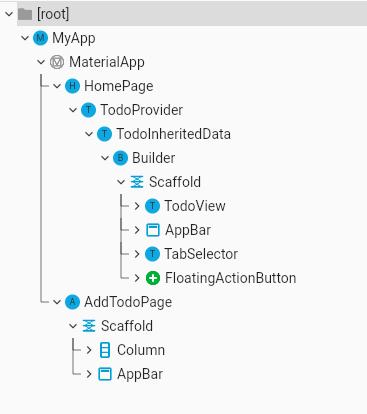
\includegraphics[width=0.6\textwidth]{Images/tree_structure_on_AddTodoPage.png}
    \caption{Shows the widgets tree structure in the AddTodoPage}
    \label{fig:add_todo_page_tree_structure}
\end{figure}


The AddTodoPage is not a part of the subtree of the HomePage but is a standalone tree. There is no instance of TodoProvider widget as ancestor of the  Scaffold widget present in the AddTodoPage. It is not possible, tough, to call the \textit{of} method as  we did before. Indeed, calling the \textit{of} method in a context where a TodoProvider widget is not present causes the assertion line (the one below) in Source Code \ref{code:2.18} to return \textit{false} and to rise a runtime error.
\mbox{}\\

\begin{code}
\begin{minted}[bgcolor=bluepoli!10]{dart}

assert(result != null, 'No TodoInheritedData found in context');
\end{minted}
\end{code}
\mbox{}\\
The easiest method to proceed is to pass the \textit{onAddTodo} function as a parameter to the AddTodoPage when it is pushed on top of the HomePage. A new parameter, called \textit{addTodoCallback }, is added to the AddTodoPage .
\mbox{}\\
\captionof{listing}{Todo app - InheritedWidget - AddTodoPage's callback function parameter creation}
\mbox{}
\begin{code}
\label{code:2.34}
\begin{minted}[bgcolor=bluepoli!10]{dart}

class AddTodoPage extends StatefulWidget {
  final void Function(String, String) addTodoCallback; // new parameter

  const AddTodoPage({Key? key, required this.addTodoCallback})
      : super(key: key);
\end{minted}
\end{code}
\mbox{}\\
Then, the MaterialApp is notified about the necessity of this new argument at the AddTodoPage creation. The argument is found inside the \textit{context}, in a specific variable called \textit{arguments.}
\mbox{}\\
\captionof{listing}{Todo app - InheritedWidget - "\textbackslash\textit{addTodo}" route parameters re-definition}
\mbox{}
\begin{code}
\label{code:2.36}
\begin{minted}[bgcolor=bluepoli!10]{dart}

routes: {
{. . .}
  "/addTodo": (context) => AddTodoPage( 
  // passing the onAddTodo functio by argument
      addTodoCallback: ModalRoute.of(context)!.settings.arguments
          as Function(String, String)),
},

\end{minted}
\end{code}
\mbox{}\\
The \textit{addTodoCallback} function is then used in the \textit{onPressed} field of the TextButton widget in the AddTodoPage. Once the TextButton is tapped, the new todo is added to the list and the AddTodoPage is popped returning to the HomePage. Being the state changed the HomePage is rebuilt.
\mbox{}\\
\captionof{listing}{Todo app - InheritedWidget - AddTodoPage \textit{onPressed }field implementation}
\mbox{}
\begin{code}
\label{code:2.36}
\begin{minted}[bgcolor=bluepoli!10]{dart}

TextButton(onPressed: () {
  widget.addTodoCallback(textControllerName.text,textControllerDesc.text);
  Navigator.pop(context);
}
\end{minted}
\end{code}
\mbox{}\\
Raising the TodoProvider widget above the MaterialApp widget would not be a good solution. The higher the TodoProvider widget resides in the tree the more widgets are rebuilt on state changes. In this case it is easier to pass the callback function as parameter to the AddTodoPage.


\paragraph{Todo updating feature - } 
\label{subpar:todo_updating_feature_inherited_wdiget}
A new function must be implemented in the TodoProvider widget and passed to the TodoInheritedData widget. This new function is called \textit{onUpdateTodo } and takes three arguments: the \textit{id} of the todo to be updated, the \textit{newName } and the \textit{newDesc}.
\mbox{}\\
\begin{code}
\captionof{listing}{Todo app - InheritedWidget - TodoProvider's \textit{onUpdateTodo }function implementation}
\mbox{}
\label{code:2.37} 
\begin{minted}[bgcolor=bluepoli!10]{dart}

  void onUpdateTodo(int id, String newName, String newDesc) {
    //control the todo's existance
    assert(todoExists(todos, id) == true, 'No todo with id : \$id');
    //create a new list with the updated todo
    List<Todo> newTodosList = todos.map((todo) {
      if (todo.id == id) {
        return Todo(
            completed: todo.completed,
            description: newDesc,
            name: newName,
            id: todo.id);
      } else {
        return todo;
      }
    }).toList();
    //update the state
    setState(() {
      todos = newTodosList;
    });
  }

\end{minted}
\end{code}
\mbox{}\\
The \textit{onUpdateTodo} function checks if a todo matching the id exists. Then, for the same immutability concept we dealt with in the previous paragraph \ref{par:feature_addition_inherited_widget}, a \textit{newTodosList }is created and populated with the elements of the \textit{todos }list. Moreover, the todo with the corresponding id is updated with the new name and the new description. Finally, the \textit{todos }list in the TodoProvider stateful widget is replaced with the \textit{newTodosList }using the \textit{setState} method.
This new \textit{onUpdateTodo} method is then made accessible down the tree adding a field to the TodoInheritedData widget.
\mbox{}\\
\begin{code}

\captionof{listing}{Todo app - InheritedWidget - \textit{onUpdateTodo} function propagation}
\mbox{}

\label{code:2.38}
\begin{minted}[bgcolor=bluepoli!10]{dart}

class TodoInheritedData extends InheritedWidget {
  
  final void Function(int, String,String) onUpdateTodo; // new variable
  final void Function(String,String) onAddTodo; 
  final List<Todo> todos;
  final List<Todo> filteredTodos;
  final void Function(VisibilityFilter) onChangeFilter;
  final int stats;
  final VisibilityFilter filter;

  (...)

class TodoProvider extends StatefulWidget {

@override
Widget build(BuildContext context) {
  return TodoInheritedData(
    todos: todos,
    onChangeFilter: onChangeFilter,
    onAddTodo: onAddTodo,
    onSetCompleted: onSetCompleted,
    onUpdateTodo: onUpdateTodo, // passing the onUpdateTodo function
    filter: filter,
    child: widget.child,
  );
}
\end{minted}
\end{code}
\mbox{}\\
For the same problem faced during the implementation of the todo addition feature, also in this case, the \textit{onUpdateTodo } function must be passed to the new route (no TodoProvider present in this context) as parameter. A new variable is added to the UpdateTodoPage, beside the already existent one, called \textit{callback }. This new variable is of type Function taking two Strings as arguments (the id will be already set up by the calling page).
\begin{code}
\mbox{}\\
\captionof{listing}{Todo app - InheritedWidget - UpdateTodoPage callback function parameter creation}
\mbox{}
\label{code:2.39}
\begin{minted}[bgcolor=bluepoli!10]{dart}

class UpdateTodoPage extends StatefulWidget {
  final Todo todo;
  final void Function(String, String) callback; // new variable

  const UpdateTodoPage({Key? key, required this.todo,
   required this.callback})
      : super(key: key);
 
 (...)
 
 \end{minted}
 \end{code}
 \mbox{}\\
We are ready now to push the UpdateTodoPage on top of the Homepage when the InkWell widget (inside the TodoItem widget) is tapped. However, there is a small extra step to perform before proceeding.  Flutter Navigator ,indeed, allows to pass a single object as argument between routes. In this case, besides the \textit{onUpdateTodo} function also a todo instance must be passed to the UpdateTodoPage. For this reason, a wrapper class is created with the name \textit{UpdateTodoPageArguments }.
\mbox{}\\
\begin{code}
\captionof{listing}{Todo app - InheritedWidget - UpdateTodoPageArguments class implementation}
\mbox{}
\label{code:2.40}
\begin{minted}[bgcolor=bluepoli!10]{dart}

class UpdateTodoPageArguments {
  final Todo todo;
  final void Function(String ,String) updateState;

  UpdateTodoPageArguments({required this.todo, required this.updateState});
}
\end{minted}
\end{code}
\mbox{}\\
Inside the InkWell’s \textit{onTap }function ,the corresponding todo and the \textit{onUpdate} function are wrapped into an object of type UpdateTodoPageArguments. This object is then passed to the new route.
\mbox{}\\
\begin{code}
\captionof{listing}{Todo app - InheritedWidget - Using a UpdateTodoPageArguments instance to pass argument between routes}
\mbox{}
\label{code:2.42}
\begin{minted}[bgcolor=bluepoli!10]{dart}

Navigator.pushNamed(context, "/updateTodo",
//passing the the state changing function using a wrapper class
    arguments: UpdateTodoPageArguments(
        todo: todo,
        updateState: (String newName,String newDesc) {
          TodoInheritedData.of(context, aspect: 0)
              .onUpdateTodo(todo.id, newName,newDesc);
        }));
\end{minted}
\end{code}
\mbox{}\\
It is necessary to specify to the MaterialApp widget where, the two parameters (necessary for the UpdateTodoPage creation), will be situated. As before , they are putted in a specific variable, inside the \textit{context} object, called \textit{arguments.}
\mbox{}\\
\begin{code}

\captionof{listing}{Todo app - InheritedWidget - "\textbackslash\textit{updateTodo}" route re-definition}
\mbox{}
\label{code:2.42}
\begin{minted}[bgcolor=bluepoli!10]{dart}

routes: {
  "/": (context) => const HomePage(),
  "/updateTodo": (context) => UpdateTodoPage(
        todo: (ModalRoute.of(context)!.settings.arguments
                as UpdateTodoPageArguments)
            .todo,
        callback:
//access the wrapper class to populate the callback parameter        
         (ModalRoute.of(context)!.settings.arguments
                as UpdateTodoPageArguments)
            .updateState,
      ),
\end{minted}
\end{code}
\mbox{}\\
Now that the \textit{onUpdateTodo }function is accessible in the UpdateTodoPage it is time to call it inside the TextButton \textit{onPressed  }field.
\mbox{}\\
\begin{code}

\captionof{listing}{Todo app - InheritedWidget - UpdateTodoPage \textit{onPressed }field implementation}
\mbox{}
\label{code:2.43}
\begin{minted}[bgcolor=bluepoli!10]{dart}

TextButton(onPressed: () {
  //call the onUpdateTodo function
  widget.callback(textControllerName.text,textControllerDesc.text);
  Navigator.pop(context);
},
\end{minted}
\end{code}
\mbox{}\\
At this point, once the user taps the confirm button, the page pops, the corresponding todo updates and the HomePage rebuilds.\\



\subsubsection{Rendering optimizations} 
\label{subpar:render_optimizations_inherited_widget}
\hfill\\
I spent some hours trying to figure out how to make the single TodoItem widget rebuild, after a non -structural change occurs. When a non-structural change occurs, may be instresting, tough, to limitate the tree rebuilding  to widgets affected by the mutation only. For example, when the Checkbox inside a TodoItem widget is tapped, would be nice to rebuild the TodoItem widget only, and not the entire TodoView widget. After some attempts, I realized that it was just not feasible using InheritedWidgets alone. InheritedWidgets, indeed, do not offer this possibility at all. Every time a widget accesses the state in the TodoProvider’s subtree, using the \textit{of} method, it is registered as \textit{listener} for state changes. Once a state change occurs ,there are only two possibilities: notify all listeners and rebuild them or notify none. In other words when a state change occurs, and it must be visualized , the entire TodoProvider’s subtree is rebuilt unconditionally. Flutter framework, however, offers a particular widget, called InheritedModel, to handle this kind of scenario. InheritedModel works as InheritedWidget except for the fact that, when a widget accesses the state ,(calling the \textit{of} method) it must provide also a new additional parameter, called \textit{aspect}. The \textit{aspect} parameter can be whatever object. For example a String or a Int, but also a more complex data structure. The \textit{aspect} parameter identifies which part (or parts) of the state the widget is registering to. 
With this new additional tool is possible to achive the partial rendering we were looking for. Indeed, with InheritedModel , widgets are rebuilt based on the changed aspect of the state. If a widget registered for a particular aspect and a state mutation, not affecting that aspect, occurs, the widget is not rebuilt. However, the entire logic defining which aspect of the data changed (when a state transition occurs) must be implemented by the programmer.\\
The extension to InheritedWidget is substituted with the extension to the InheritedModel, in the
TodoInheritedData class.
\mbox{}\\
\begin{code}
\captionof{listing}{Todo app - InheritedModel - extension to InheritedModel }
\mbox{}
\label{code:2.44}
\begin{minted}[bgcolor=bluepoli!10]{dart}

class TodoInheritedData extends InheritedModel<int> {
\end{minted}
\end{code}
\mbox{}\\
I decided to use Ints in order to identify aspects. In particular, widgets that need to rebuild on \textit{filteredTodos} list structural change, register to the aspect identified with the number 0. Widgets that do always need to rebuild register to the aspect identified with number 1. Widgets that need to rebuild when a non-structural change, affecting the specific Todo with id n, occurs register to the aspect identified with the number n. (no Todos will have id with value 0 or 1. This is a convention I used to keep things simple. Other ,more complex structure , could be used to avoid this behaviour). 
At this point, the \textit{of} method, contained in the TodoInheritedData widget, should be updated taking into account the \textit{aspect} parameter. Morevover, the \textit{result} variable should be populated with the \textit{inheritedFrom} static method belonging to the InheritedModel class, instead of the \textit{dependOnInheritedWidgetOfExactType} static method belonging to InheritedWidget class.
\mbox{}\\
\begin{code}
\captionof{listing}{Todo app - InheritedModel - TodoInheritedData's  \textit{of} method implementation}\mbox{}
\label{code:2.45}
\begin{minted}[bgcolor=bluepoli!10]{dart}
//add the aspect argument
static TodoInheritedData of(BuildContext context, {required int aspect})
 {
  final TodoInheritedData? result =
  //calling the inheritFrom method using the aspect parameter
      InheritedModel.inheritFrom<TodoInheritedData>(context,
       aspect: aspect);
  assert(result != null, 'No TodoInheritedData found in context');
  return result!;
}
\end{minted}
\end{code}
\mbox{}\\
All the lines of code accessing the state with the \textit{of} method must now be changed taking into account the new implementation and the new \textit{aspect} argument.
\mbox{}\\

\begin{code}
\label{code:2.47}
\begin{minted}[bgcolor=bluepoli!10]{dart}

TodoInheritedData.of(context, aspect: aspect)
\end{minted}
\end{code}
\mbox{}\\
In particular, the TodoView widget will pass as \textit{aspect} argument the number 0 declaring that should be notified (and rebuild) only when a structural change occurs.
Instead, TodoItem widgets will pass the corresponding Todo’s \textit{id} in the \textit{aspect} parameter.
Now that every widget is registered to the desired aspect of the data, it is necessary to “teach” the TodoInheritedData widget to recognize aspects' changes. To do so, InheritedModel provides a method called \textit{updateShouldNotifyDepenedent} that is similar to the InheritedWidget’s one, \textit{updateShouldNotify }, but takes as argument also a Set of ints called \textit{dependencies }  (aspects). Once a transition occurs this method is called once for every widget that registered to state's changes. The \textit{dependencies }  variable will contain all the \textit{aspects} the widget registered to (only one for every widget in our case). Before proceeding with the \textit{updateShouldNotifyDepenedent} method's implementation we define a function called \textit{\_checkStructuralChange} that check if two lists have strctural differences.
\mbox{}\\
\begin{code}
\captionof{listing}{Todo app - InheritedModel - TodoInheritedData's \textit{updateShouldNotifyDepented} method implementation}\mbox{}
\label{code:2.46}
\begin{minted}[bgcolor=bluepoli!10]{dart}
 bool _checkStructuralChange(List<Todo> before, List<Todo> current) {
    //calculate the length of the current filtered list
    int currLen = current.length;
    //calculate the length of the previous filtered list
    int prevLen = before.length;

    bool structureRebuildLen = (currLen != prevLen);
    //check if the two lengths differ
    if (structureRebuildLen) {
      // if they differ a structural change occured
      return true;
    } else {
      //map the current list to a list containing the ids only
      List<int> currIds = current.map((todo) => todo.id).toList();
      //map the previous list to a list containing the ids only
      List<int> prevIds = before.map((todo) => todo.id).toList();
      //check they are the same
      bool sameIds = listEquals(currIds, prevIds);
      if (!sameIds) {
        //if they differ a structural change uccurred
        return true;
      } else {
        // no structural change occured
        return false;
      }
    }
  }
  @override
  bool updateShouldNotifyDependent(
      TodoInheritedData oldWidget, Set<int> dependencies) {
    if (dependencies.contains(1)) {
    // the widget do always need to rebuild
      return true;
    }
    if (dependencies.contains(0)) {
    //widget registered for structural changes
      bool structuralChange =
          _checkStructuralChange(oldWidget.filteredTodos, filteredTodos);
      if (structuralChange) {
      //in case structural changes occurred
        return true;
      } else {
        return false;
      }
    }
    //if this point is reached the widget registered    
    //for a particular todo's changes
    //check if that todo changed
    List<bool> components = [];
    for (var element in filteredTodos) {
      components.add(dependencies.contains(element.id) &&
          !oldWidget.filteredTodos.contains(element));
    }
    bool res = components.fold(
        false, (bool previousValue, bool element) => previousValue || element);
    return res;
  }
\end{minted}
\end{code}
\mbox{}\\
This method was tough to code. The method's pseudocode is presented down below. 
\mbox{}\\
\begin{code}
\captionof{listing}{Todo app - InheritedModel - TodoInheritedData's \textit{updateShouldNotifyDepented} method pseudocode}
\mbox{}
\label{code:2.48}
\begin{minted}[bgcolor=bluepoli!10]{dart}
if( widgetRegisteredForStructuralChange && strucuturalChangeOccured){
        return true;
    }else{
        if( widgetRegisteredForSpecificTodoChange && thatTodoChanged){
            return true;
            }else{
                return false;
    }
}
\end{minted}
\end{code}
\mbox{}\\
I propose now two pratical examples to clearify a bit the  \textit{updateShouldNotifyDepenedent} behaviour.
\paragraph{Pratical example 1 - } 
\label{subpar:todo_updating_feature_inherited_wdiget}
Suppose to have a list of todos containing two todo instances, one with id 38 and one with id 121. In the HomePage there is a TodoView widget containing two TodoItem widgets. TodoView widget calls the \textit{of} method in order to access the state passing the int value 0 as parameter. The two TodoItem widgets call the \textit{of} method in order to access the state passing their todo's id value as parameter. Suppose now to add a new todo in the list using the AddTodoPage. The \textit{updateShouldNotifyDepented} method is called once for every widget that access the state. Note that also the TabSelector and the VisibilityFilterSelector widgets access the state using the \textit{of} method but their are not considered in this example. So, the \textit{updateShouldNotifyDepenedent} method is called once for the TodoView widget, with dependencies value equal to 0. It is also called once for every TodoItem widget with dependencies value equal to 38, in one case, and equal to 121, in the other. Before actually rebuilding any widget the framework executes all the \textit{updateShouldNotifyDepenedent} method calls. We start analizing the call for the TodoItem widget with id 38 with reference to the pseudocode defined in Source Code \ref{code:2.48}. In this case a structural change occured ( we added a todo)  but the widget did not registered for structural changes ( dependencies do not contains 0). Moreover, the widget registered for changes in the todo with id 38 but no changes occured in that todo. The function returns false and the widget is not rebuilt. The same happens for the \textit{updateShouldNotifyDepenedent} methods execution of the TodoItem widget with id 121. In the \textit{updateShouldNotifyDepenedent} method execution for the TodoView widget, instead, the dependencies list contains the value 0(and only that). In this case the TodoView widget registered for structural changes and a structural change occured (the new list is longer than the old one). The \textit{updateShouldNotifyDepenedent} method returns true and the widget is rebuilt creating a new TodoView widget composed by three TodoItem widgets this time.
\paragraph{Pratical example 2 - } 
\label{subpar:todo_updating_feature_inherited_wdiget}
Suppose to have a list of todos containing two todo instances as before, one with id 38 and one with id 121. In the HomePage there is a TodoView widget containing two TodoItem widgets. TodoView widget calls the \textit{of} method in order to access the state passing the int value 0 as parameter. The two TodoItem widgets call the \textit{of} method in order to access the state passing their corresponding todo's id value as parameter. Suppose now to tap on the TodoItem widget's checkbox with id 38 in order to change its \textit{completed} value. As before the \textit{updateShouldNotifyDepenedent} method is called once for every widget that access the state. The \textit{updateShouldNotifyDepenedent} method execution regarding the TodoView widget returns false because the second if in the Source Code \ref{code:2.48} evaluates to false due to the fact that the widget did not registered for specific todo's changes. The TodoView widget is not rebuilt then. In the \textit{updateShouldNotifyDepenedent} method execution regarding the TodoItem widget with id 121 the part that leads the entire method to return false is the second expression in the second if statement. Indeed, the todo with id 121 did not changed with respect to the one contained in the previous state. The TodoItem widget with is 121 is consequently not rebuilt. The execution of the \textit{updateShouldNotifyDepenedent} method concerning the TodoItem with id 38, instead, return true. The second condition is, indeed, satisfied by the fact that the widget registered for a specific todo's change and also that todo changed. The todo with id 38 is, indeed, changed with respect to the todo with id 38 in the previous state. This leads the TodoItem widget with id 38 to rebuild leaving all the other widgets unchanged.


\mbox{}\\

At this point , when the TodoItem’s checkbox is tapped the single TodoItem widget is rebuilt. However, no visual changes are shown. The widget rebuilds with the same information as before . This is due to the fact that, the \textit{build} method, populates its internal widgets based on a local \textit{todo} variable. This variable is populated on the TodoItem widget's creation with a Todo instance provided by the parent widget(TodoView). Indeed, when the TodoView widget instantiates TodoItems  in its ListView, it creates a copy of the corresponding Todo before passing it to the constructor. Even if we changed the information contained in the TodoInheritedData widget, the TodoItem widget do not see any difference.  Its local todo variable , indeed, did not change. The fact that, before the optimizations, TodoItem widgets rebuilt correctly comes from the fact that every transition of the state caused the entire TodoView widget to rebuild. The conseguence was that TodoItems were detroyed and created again using new copies of the data coming from the TodoInheritedData widget. \\
To recap, the performance optimization we were looking for were achieved succesfully but an issue ,regarding the syncronization of the data, arised. The TodoItems widget sees a screenshot of the state different from the one seen by the rest of the application. This is a really bad behavior and is caused by the fact that ,sometimes, during programming , more than one level of information caching is required or used to avoid effort in coding and performance issues. In other words, a local copy of the data is kept and referred to in case of data access in order to optimize the accesses in the main storage that can become quite expensive in large scenarios. A great example of that is the local copy of the database’s data used in many applications. Is more effective to fetch data from the database, save them locally, manipulate this local copy and only in case of real necessity access again the database to store them or retrieve other data. In large applications (but also in small ones like in this cases) more than one level of data caching is used. Particular attention is required to handle those levels to avoid inconsistency in what is visualized and the real data. In this case the \textit{filteredTodos} list actually changed but the UI did not reflect this change. The problem was generate by the fact that a local copy of the real Todo instance was passed to the TodoItem widget. Instead , the "correct" way of handling this scenario is to pass the id of the Todo in the constructor and then use this id to look up for the Todo instance in the centralized state (the TodoInheritedData). This of course will require more computational effort but  will guarantee also a lot more stability and robustness. 
Therefore, TodoItem widget's local variable of type Todo is replaced with a new int variable called \textit{id} that represents the id of the Todo the widget is visualizing. In the \textit{build} method, then, the corresponding Todo is looked up.

\mbox{}\\
\begin{code}
\captionof{listing}{Todo app - InheritedModel - accesing the state into TodoItem component}

\label{code:2.48}
\begin{minted}[bgcolor=bluepoli!10]{dart}
class TodoItem extends StatelessWidget {
  final int id; // Todo variable replaced with a int one

  const TodoItem({Key? key, required this.id}) : super(key: key);

  @override
  Widget build(BuildContext context) {
  	// getting the todo instance from the state
    final Todo todo = TodoInheritedData.of(context, aspect: id)
        .todos
        .where((element) => element.id == id)
        .first;
\end{minted}
\end{code}
\mbox{}\\
At this point I also suggest to generate a new unique Key, in the TodoView widget, and pass it to the TodoItem widget. I indeed faced a "strange" bug/behaviour before providing a unique key to every TodoItem widgets. This bug showed up performing multiple filter changes and subsequently performing a todo update regarding the \textit{completed  }field (but also in case of other updates I suppose). In that case not only the interested TodoItem widget rebuilt but also other, apparently random, ones. Investigating a bit I discovered that some TodoItem widgets turned out to be registered for more than one aspect after the filter changes. This was clearly not possible because every TodoItem widget registers for a single aspect by construction. The only reason I could think of was that some of them were reused by the framework to avoid discarding them and rebuilding them from scratch. Indeed, when the TodoView is rebuilt multiple times in a single execution the Flutter framework tries to minimize the creation of TodoItem widgets. I did not understood in depth where this bug was generated but it was solved right after I added a unique key to every TodoItem widget. Providing a unique key blocks the framework from reusing TodoItem instances. 
After this adjunctive passage the application is working as intentioned and the rendering optimizations were successfully accomplished. \\


\subsubsection{Conclusions} 
\label{subpar:render_optimizations_inherited_widget}
Table \ref{table:recap_inheritedwidgets} reports some measurements taken from the InheritedWidget's implementation process. The \textit{lines of code} column represents the lines of code added or updated with respect to the shared project structure proposed in subsection \ref{subsec:todo_app_shared_project_structure}. The \textit{time }column represents the time spent in order to implement the corresponding subprocess. The unit of measure \textbf{h} stands for hours and \textbf{m} stands for minutes. The \textit{lines-time ratio} column represents the average number of lines written in a minute. The \textit{classes} column represents the number of created classes in each subprocess.
\begin{table}[H]
    \caption*{\textbf{Measurement for InheritedWidget process}}
    \centering 
    
    \begin{tabular}{| l | c | c | c | c |}
    \hline
    \rowcolor{bluepoli!40} % comment this line to remove the color
    \hline
     & \textbf{lines of code} & \textbf{time} & \textbf{lines/time ratio} & \textbf{classes} \T\B \\
     \hline
    \textbf{base functionalities} & 100 & 2-3 h & 0.66 l/m & 2  \T\B \\ 
    \textbf{feature addition} & 58 & 20-30 m & 2.32 l/m & 1 \T\B\\ 
    \textbf{rendering optimization} & 45 & 8-10 h & 0.084  l/m & 0 \B\\
    \hline
    \end{tabular}
    \\[10pt]
    \caption{InheritedWidget measurements table}
    \label{table:recap_inheritedwidgets}
\end{table}

Figure \ref{image:inheritedwidgets_lines_piechart} represents a pie chart showing the percentage of lines of code written in each implementation's process, including the one regarding the shared structure. The whole process is quite balanced in term of lines of code. The 64\% of the code is used to produce the presentation layer and the remaining 36\% is used to manage the state and its optimizations. Considering the fact that the UI is kept minimal truncating the necessary lines of code accentuates even more the fact that the state management took less than a half of the entire written code. 

\begin{figure}[H]
\caption*{\textbf{Lines}}
\centering
\begin{tikzpicture}

\pie[rotate =0 ]{62/Shared structure - 302,
    19/Base functionalities - 100,
    11.5/Feature addition - 58,
    9.5/Optimizations - 45
    }
 
\end{tikzpicture}
 \caption{Shows the pie chart regarding the lines of code spent in each subprocess for the InheritedWidget implementation}
\label{image:inheritedwidgets_lines_piechart}
\end{figure}

Figure \ref{image:inheritedwidgets_hours_piechart} represents a pie chart showing the percentage of time spent in each implementation's process. Notice that the optimizations process took more than the 75\% of the entire time.
\begin{figure}[H]
 \caption*{\textbf{Hours}}
\centering
\begin{tikzpicture}

\pie[rotate = 90]{
    20.97/Base functionalities ,
    3.49/Feature addition,
    75.52/Optimizations 
    }

\end{tikzpicture}
 \caption{Shows the pie chart regarding the hours spent in each subprocess for the InheritedWidget implementation}
 \label{image:inheritedwidgets_hours_piechart}
\end{figure}

Figure \ref{fig:struttura_cartelle_inherited} shows the final folders structure for the InheritedWidget implementation. The only  file added to the original folders structure is the todo\_provider.dart file.

\begin{figure}[H]
    \centering
    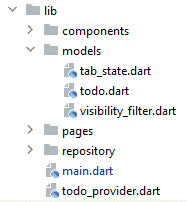
\includegraphics[width=0.4\textwidth]{Images/struttura_cartelle_inherited.png}
    \caption{Shows the final folders structure for the InheritedWidget implementation of the Todos app}
    \label{fig:struttura_cartelle_inherited}
\end{figure}

Figure \ref{fig:widget_tree_structure_inheritedwidget} represents the widget's tree structure for the InheritedWidget final application. Notice the TodoProvider widget, situated below the HomePage, providing an instance of the TodoInheritedData to the subtree.

\begin{figure}[H]
    \centering
    \subfloat[Widgets tree structure \textit{todos }tab \label{fig:widget_tree_structure_todostab_inheritedwidget}]{
        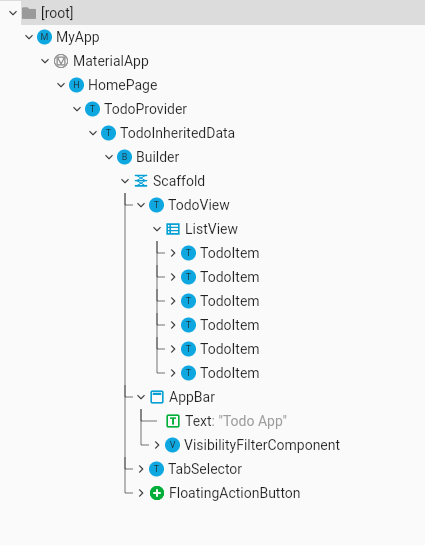
\includegraphics[scale=0.6]{Images/albero_inherited_todos.png}
    }
    \quad
    \subfloat[Widgets tree structure \textit{stats }tab\label{fig:widget_tree_structure_todostab_inheritedwidget}]{
        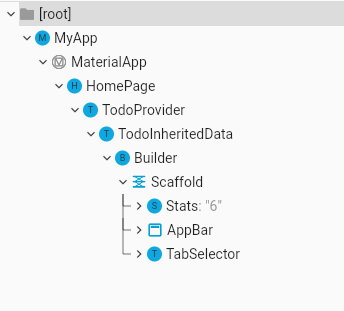
\includegraphics[scale=0.6]{Images/albero_inherited_stats.png}
    }
    \caption{Shows the widgets tree structure for InhritedWidget Todos app}
    \label{fig:widget_tree_structure_inheritedwidget}
\end{figure}

\subsection{Redux implementation}
\subsection{BloC implementation}
\subsection{MobX implementation}
\subsection{GetX implementation}




\chapter{The Other app}
\label{ch:chapter_three}%
Another app developed using same state managemnts solutions
\chapter{Comparisons}
\label{ch:comparisons}
Some comparisons involving the data i kept and the other word file i have sent to you before
\chapter{Conslusions}
\label{ch:conclusion}
Conclusions 
%-------------------------------------------------------------------------
%	BIBLIOGRAPHY
%-------------------------------------------------------------------------

\addtocontents{toc}{\vspace{2em}} % Add a gap in the Contents, for aesthetics
\bibliography{Thesis_bibliography} % The references information are stored in the file named "Thesis_bibliography.bib"

%-------------------------------------------------------------------------
%	APPENDICES
%-------------------------------------------------------------------------

\cleardoublepage
\addtocontents{toc}{\vspace{2em}} % Add a gap in the Contents, for aesthetics
\appendix
\chapter{Appendix A}
If you need to include an appendix to support the research in your thesis, you can place it at the end of the manuscript.
An appendix contains supplementary material (figures, tables, data, codes, mathematical proofs, surveys, \dots)
which supplement the main results contained in the previous chapters.

\chapter{Appendix B}
It may be necessary to include another appendix to better organize the presentation of supplementary material.


% LIST OF FIGURES
\listoffigures

% LIST OF TABLES
\listoftables

\renewcommand\lstlistlistingname{List of source codes}
\lstlistoflistings
% ACKNOWLEDGEMENTS
\chapter*{Acknowledgements}
Here you might want to acknowledge someone.

\cleardoublepage

\end{document}
